\documentclass[../main.tex]{subfiles}
\begin{document}
Java è un linguaggio di programmazione fortemente tipicizzato, ogni variabile e ogni espressione ha un tipo conosciuto al momento 
della compilazione. Ecco uno schema con i principali tipi di dato:
\begin{figure}[h]
    \centering
    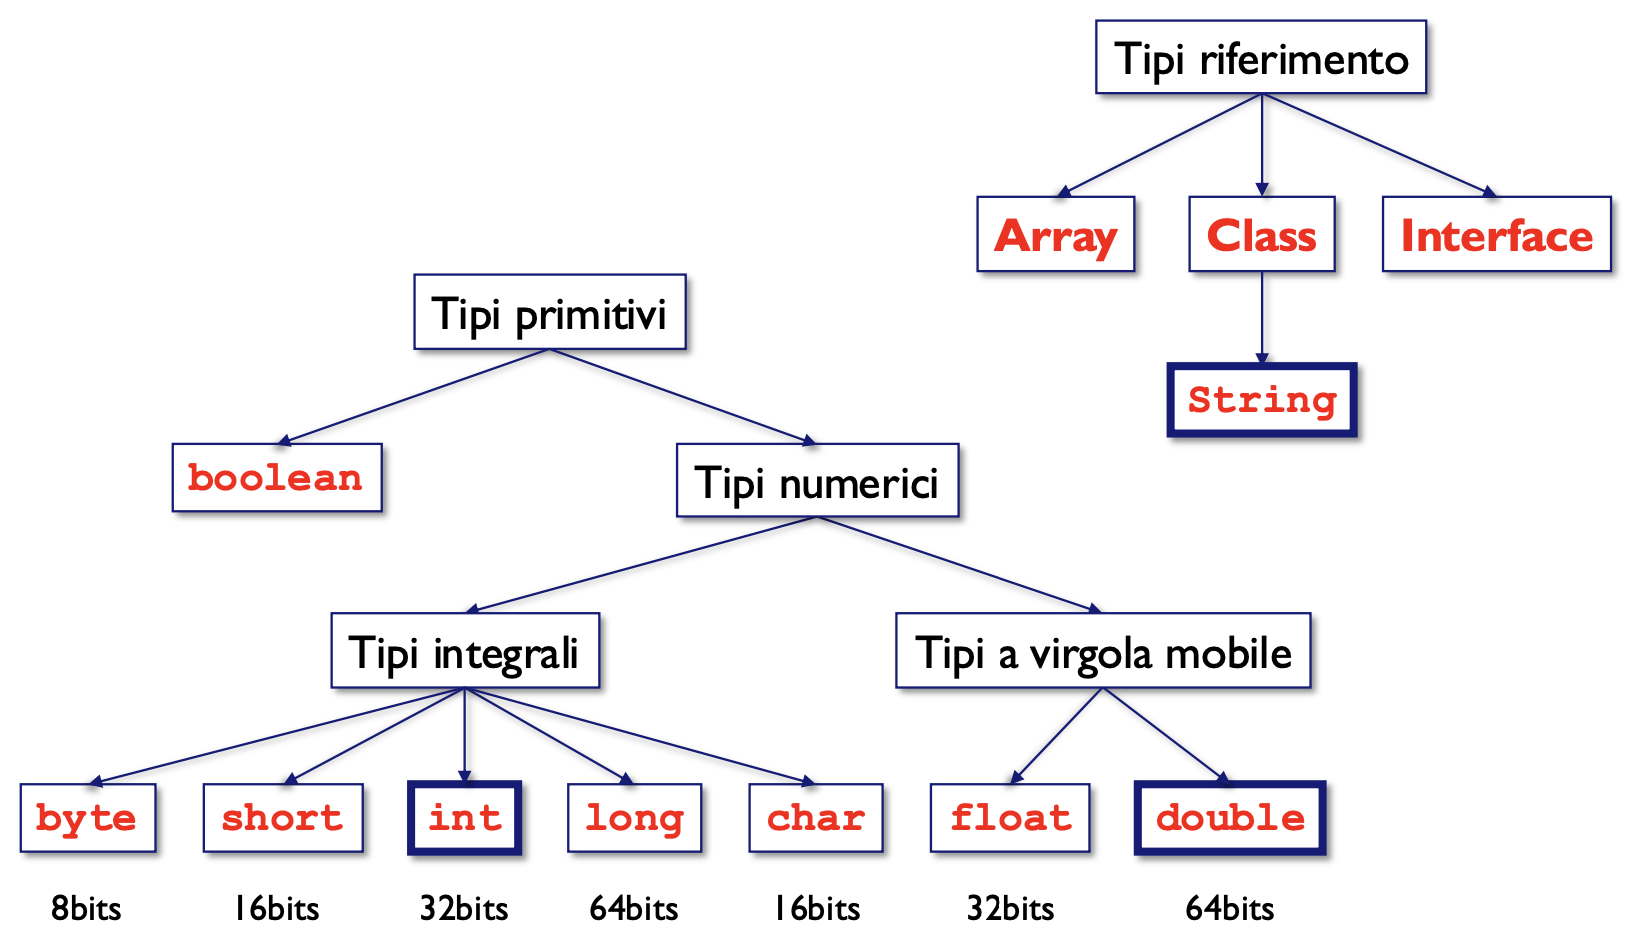
\includegraphics[width=1\textwidth]{../images/tipiDato.png}
\end{figure}

\subsection{boolean}
Il tipo \code{boolean} può assumere esclusivamente due valori: \code{true} e \code{false}. I valori booleani si ottengono anche dalla
valutazione di espressioni condizionali, ad esempio:
\begin{lstlisting}[style=java]
    boolean risultato = tasso > 0.05;
\end{lstlisting}

\subsection{Tipi numerici}
\subsubsection{Interi}
I tipi numerici interi sono rispettivamente \code{byte}, \code{short}, \code{int} e \code{long}. L'unica differenza tra di essi
è il range di numeri che è possibile rappresentare. Per valori ancora più grandi è possibile utilizzare il tipo di dato
\code{java.math.BigInteger}.

\subsubsection{char}
Serve per rappresentare i singoli caratteri. Esso permette l'utilizzo dei caratteri \textbf{Unicode}, uno standard per la rappresentazione
consistente del testo. Ad ogni carattere è assegnato un valore numerico ed è quindi possibile fare operazioni aritmetiche sui caratteri.

\subsubsection{Decimali}
È molto raro, ma ci sono alcuni numeri decimali che non possono essere rappresentati. In generale per comparare due valori decimali
non utilizziamo \code{==}:
\begin{lstlisting}[style=java]
    static final double EPSILON = 1e-8; //1 * 10^-8
    if(Math.abs(a-b) < EPSILON) { //confronta a e b
        ...
    }
\end{lstlisting}
I tipi decimali utilizzati solitamente sono \code{float} e \code{double}, per valori ancora più grandi è possibile utilizzare il tipo
di dato \code{java.math.BigDecimal}.

\subsection{Operatori logici}
Per eseguire operazioni con valori di tipo \code{boolean}:
\begin{itemize}
    \item \code{\&\&} and
    \item \code{||} or
    \item \code{!} not
    \item \code{\^} xor
\end{itemize}

\textbf{Nota:} Gli operatori \code{\&\&} e \code{||} sono \underline{cortocircuitati}. Significa che la seconda espressione viene 
valutata solo se necessario. Ad esempio:
\begin{lstlisting}[style=java]
    (x != 0) && (y / x > 1)
\end{lstlisting}
Se \code{x = 0} allora la condizione \code{x != 0} restituisce \code{false} ed è inutile (oltre che dannoso) verificare anche la seconda
condizione.

\subsubsection{Algebra di Boole}
Proprietà dell'algerbra:
\begin{itemize}
    \item \textbf{commutativa:}
    \begin{lstlisting}[style=java]
        A && B = B && A
        A || B = B || A
    \end{lstlisting}
    \item \textbf{associativa:}
    \begin{lstlisting}[style=java]
        (A && B) && C = A && (B && C)
        (A || B) || C = A || (B || C)
    \end{lstlisting}
    \item \textbf{idempotenza:}
    \begin{lstlisting}[style=java]
        A && A = A
        A || A = A
    \end{lstlisting}
    \item \textbf{assorbimento:}
    \begin{lstlisting}[style=java]
        A && (A || B) = A
        A || (A && B) = A
    \end{lstlisting}
    \item \textbf{distributiva:}
    \begin{lstlisting}[style=java]
        A && (B || C) = (A && B) || (A && C)
        A || (B && C) = (A || B) && (A || C)
    \end{lstlisting}
    \item \textbf{esistenza di minimo e massimo:}
    \begin{lstlisting}[style=java]
        A && false = false
        A || true = true
    \end{lstlisting}
    \item \textbf{esistenza del complemento:}
    \begin{lstlisting}[style=java]
        A && (!A) = false
        A || (!A) = true
    \end{lstlisting}
    \item \textbf{teoremi di DeMorgan:}
    \begin{lstlisting}[style=java]
        !(A && B) = (!A) || (!B)
        !(A || B) = (!A) && (!B)
    \end{lstlisting}
\end{itemize}

\vspace{1cm}
\subsection{Operatori aritmetici}
Si applicano a tutti i \textbf{tipi numerici:}
\begin{itemize}
    \item \code{+} addizione
    \item \code{-} sottrazione
    \item \code{*} moltiplicazione
    \item \code{/} divisione
    \item \code{\%} modulo (resto della divisione)
\end{itemize}

\subsubsection{Operatori \code{++} e \code{--}}
L'operazione \code{x = x + 1} può essere scritta come \code{x++}.
L'operazione \code{x = x - 1} può essere scritta come \code{x--}.

\begin{itemize}
    \item Operatore postfisso \code{x++}, prima valuto \code{x} e poi incremento
    \item Operatore prefisso \code{++x}, prima incremento \code{x} e poi valuto
\end{itemize}

\vspace{1cm}
\subsection{Letterali}
Un letterale è la rappresentazione di un valore di tipo primitivo, una stringa o il valore \code{null}.

\textbf{Nota:} un letterale è di tipo \code{double} \underline{solo} se contiene la virgola (\code{5.}), altrimenti è di tipo \code{int}.

\textbf{Nota:} un letterale è di tipo \code{long} \underline{solo} se termina con la lettera \code{l} o \code{L},
altrimenti è di tipo \code{int}.

\textbf{Nota:} un letterale è di tipo \code{float} \underline{solo} se termina con la lettera \code{f} o \code{F},
altrimenti è di tipo \code{double}.

\vspace{1cm}
\subsection{Conversioni}
Le conversioni \textbf{implicite} vengono effettuate automaticamente dal compilatore. Esse avvengono nel caso si passi da un tipo di dato
più piccolo \underline{ad uno più grande} o da un tipo di dato con una precisione minore \underline{ad uno con la precisione maggiore}.
\begin{figure}[h]
    \centering
    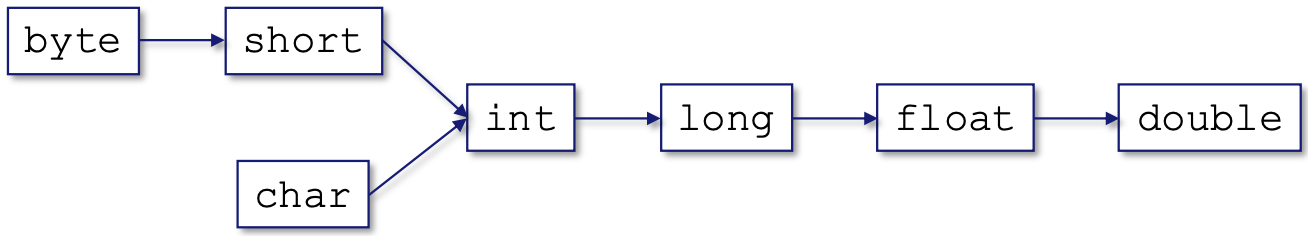
\includegraphics[width=0.8\textwidth]{../images/conversioni.png}
\end{figure}

\textbf{Nota:} le conversioni \textbf{esplicite}, vanno al contrario rispetto allo schema.


\end{document}